\documentclass[ignorenonframetext,]{beamer}
\setbeamertemplate{caption}[numbered]
\setbeamertemplate{caption label separator}{: }
\setbeamercolor{caption name}{fg=normal text.fg}
\beamertemplatenavigationsymbolsempty
\usepackage{lmodern}
\usepackage{amssymb,amsmath}
\usepackage{ifxetex,ifluatex}
\usepackage{fixltx2e} % provides \textsubscript
\ifnum 0\ifxetex 1\fi\ifluatex 1\fi=0 % if pdftex
  \usepackage[T1]{fontenc}
  \usepackage[utf8]{inputenc}
\else % if luatex or xelatex
  \ifxetex
    \usepackage{mathspec}
  \else
    \usepackage{fontspec}
  \fi
  \defaultfontfeatures{Ligatures=TeX,Scale=MatchLowercase}
\fi
\usecolortheme{seahorse}
\usefonttheme{structurebold}
% use upquote if available, for straight quotes in verbatim environments
\IfFileExists{upquote.sty}{\usepackage{upquote}}{}
% use microtype if available
\IfFileExists{microtype.sty}{%
\usepackage{microtype}
\UseMicrotypeSet[protrusion]{basicmath} % disable protrusion for tt fonts
}{}
\newif\ifbibliography
\hypersetup{
            pdftitle={Usando y Enseñando R para Investigación Reproducible},
            pdfborder={0 0 0},
            breaklinks=true}
\urlstyle{same}  % don't use monospace font for urls
\usepackage{graphicx,grffile}
\makeatletter
\def\maxwidth{\ifdim\Gin@nat@width>\linewidth\linewidth\else\Gin@nat@width\fi}
\def\maxheight{\ifdim\Gin@nat@height>\textheight0.8\textheight\else\Gin@nat@height\fi}
\makeatother
% Scale images if necessary, so that they will not overflow the page
% margins by default, and it is still possible to overwrite the defaults
% using explicit options in \includegraphics[width, height, ...]{}
\setkeys{Gin}{width=\maxwidth,height=\maxheight,keepaspectratio}

% Prevent slide breaks in the middle of a paragraph:
\widowpenalties 1 10000
\raggedbottom

\AtBeginPart{
  \let\insertpartnumber\relax
  \let\partname\relax
  \frame{\partpage}
}
\AtBeginSection{
  \ifbibliography
  \else
    \let\insertsectionnumber\relax
    \let\sectionname\relax
    \frame{\sectionpage}
  \fi
}
\AtBeginSubsection{
  \let\insertsubsectionnumber\relax
  \let\subsectionname\relax
  \frame{\subsectionpage}
}

\setlength{\parindent}{0pt}
\setlength{\parskip}{6pt plus 2pt minus 1pt}
\setlength{\emergencystretch}{3em}  % prevent overfull lines
\providecommand{\tightlist}{%
  \setlength{\itemsep}{0pt}\setlength{\parskip}{0pt}}
\setcounter{secnumdepth}{0}
\setbeamertemplate{navigation symbols}{}
\setbeamertemplate{footline}[page number]

\title{Usando y Enseñando R para Investigación Reproducible}
\author{Rayna M. Harris\\
Twitter y Instagram y GitHub: @raynamharris\\
Página web: \url{https://raynamharris.github.io}\\}
\date{27 Marzo 2018\\
R-Ladies Buenos Aires}

\begin{document}
\frame{\titlepage}

\begin{frame}{La programación es importante porque permite automatizar
tareas.}

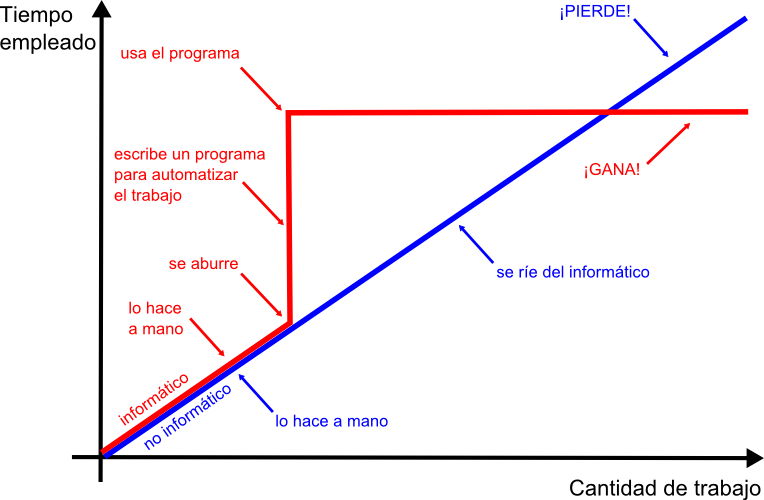
\includegraphics[width=0.75000\textwidth]{../figures/10_talk/trabajo-tiempo-8.png}
\footnote<.->{\url{http://www.mclibre.org/consultar/python/otros/lenguajes-programacion.html}}

\end{frame}

\begin{frame}{R permite estadísticas reproducibles y visualización de
datos}

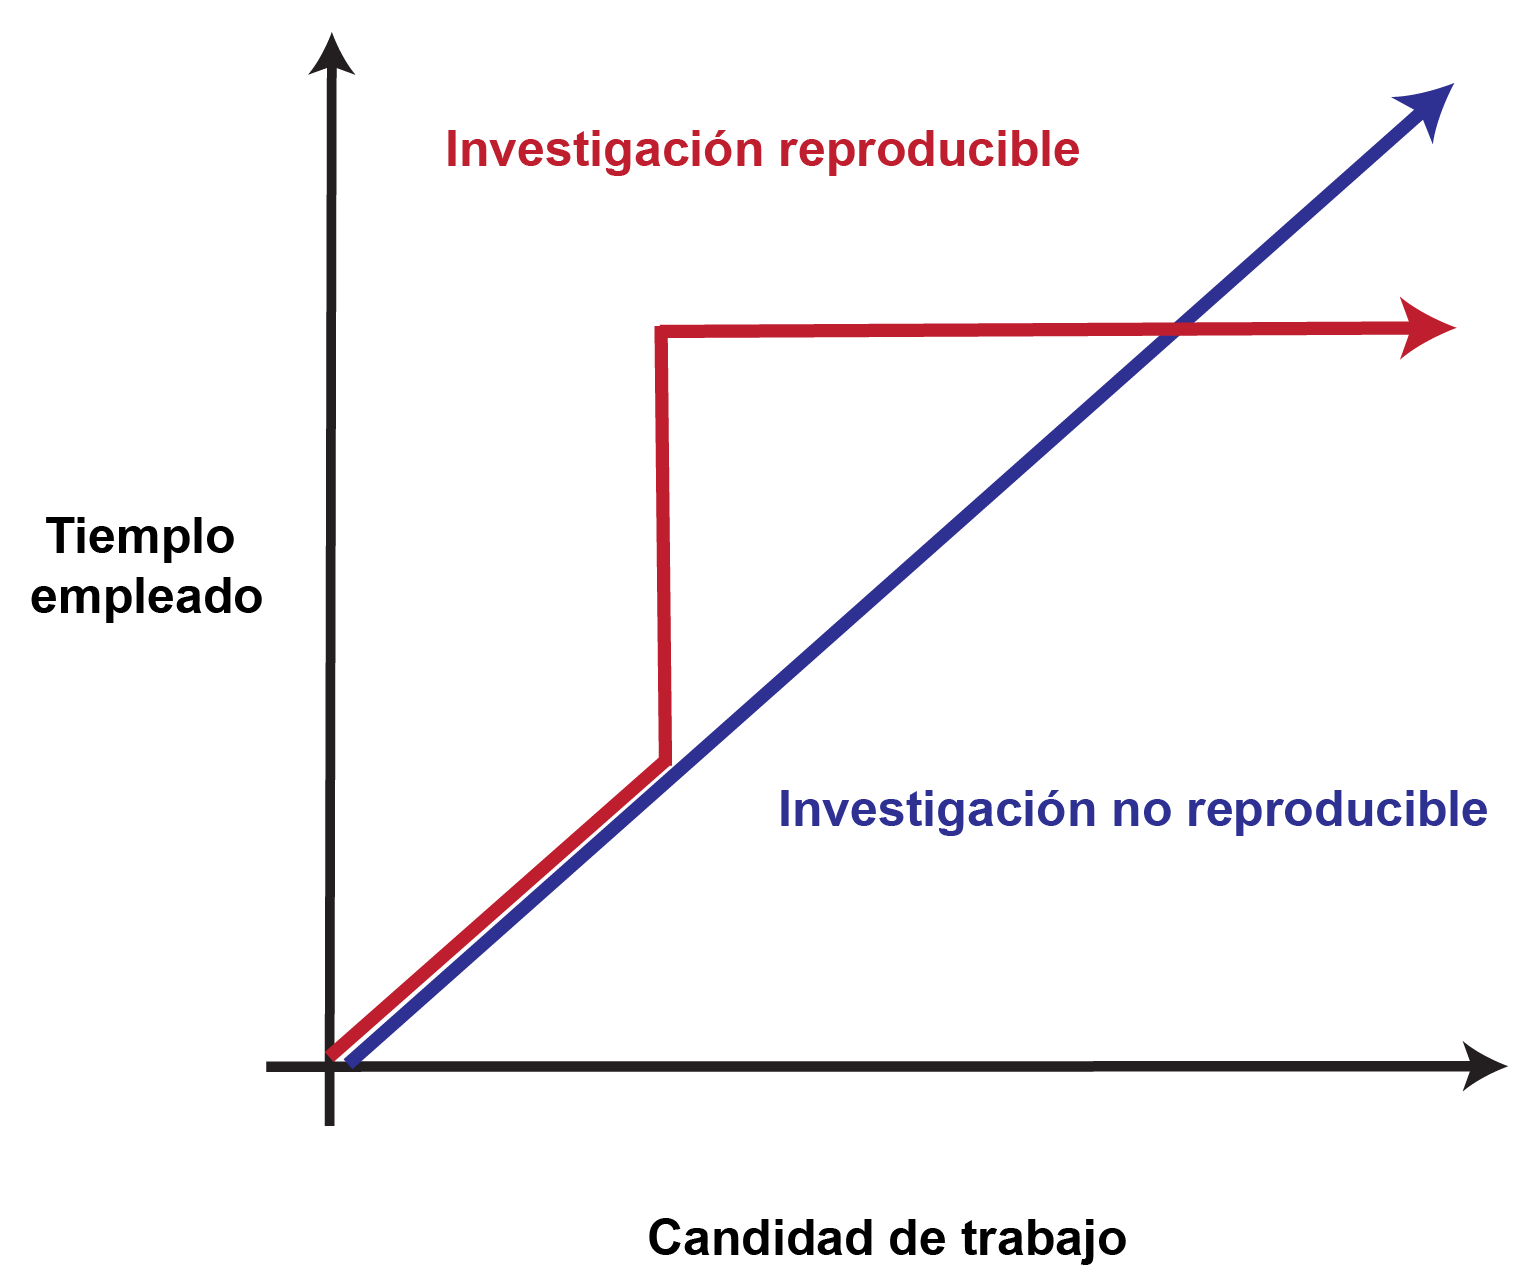
\includegraphics[width=0.75000\textwidth]{../figures/10_talk/tiempo-01.png}

\end{frame}

\begin{frame}{La enseñanza colaborativa también ahorra tiempo}

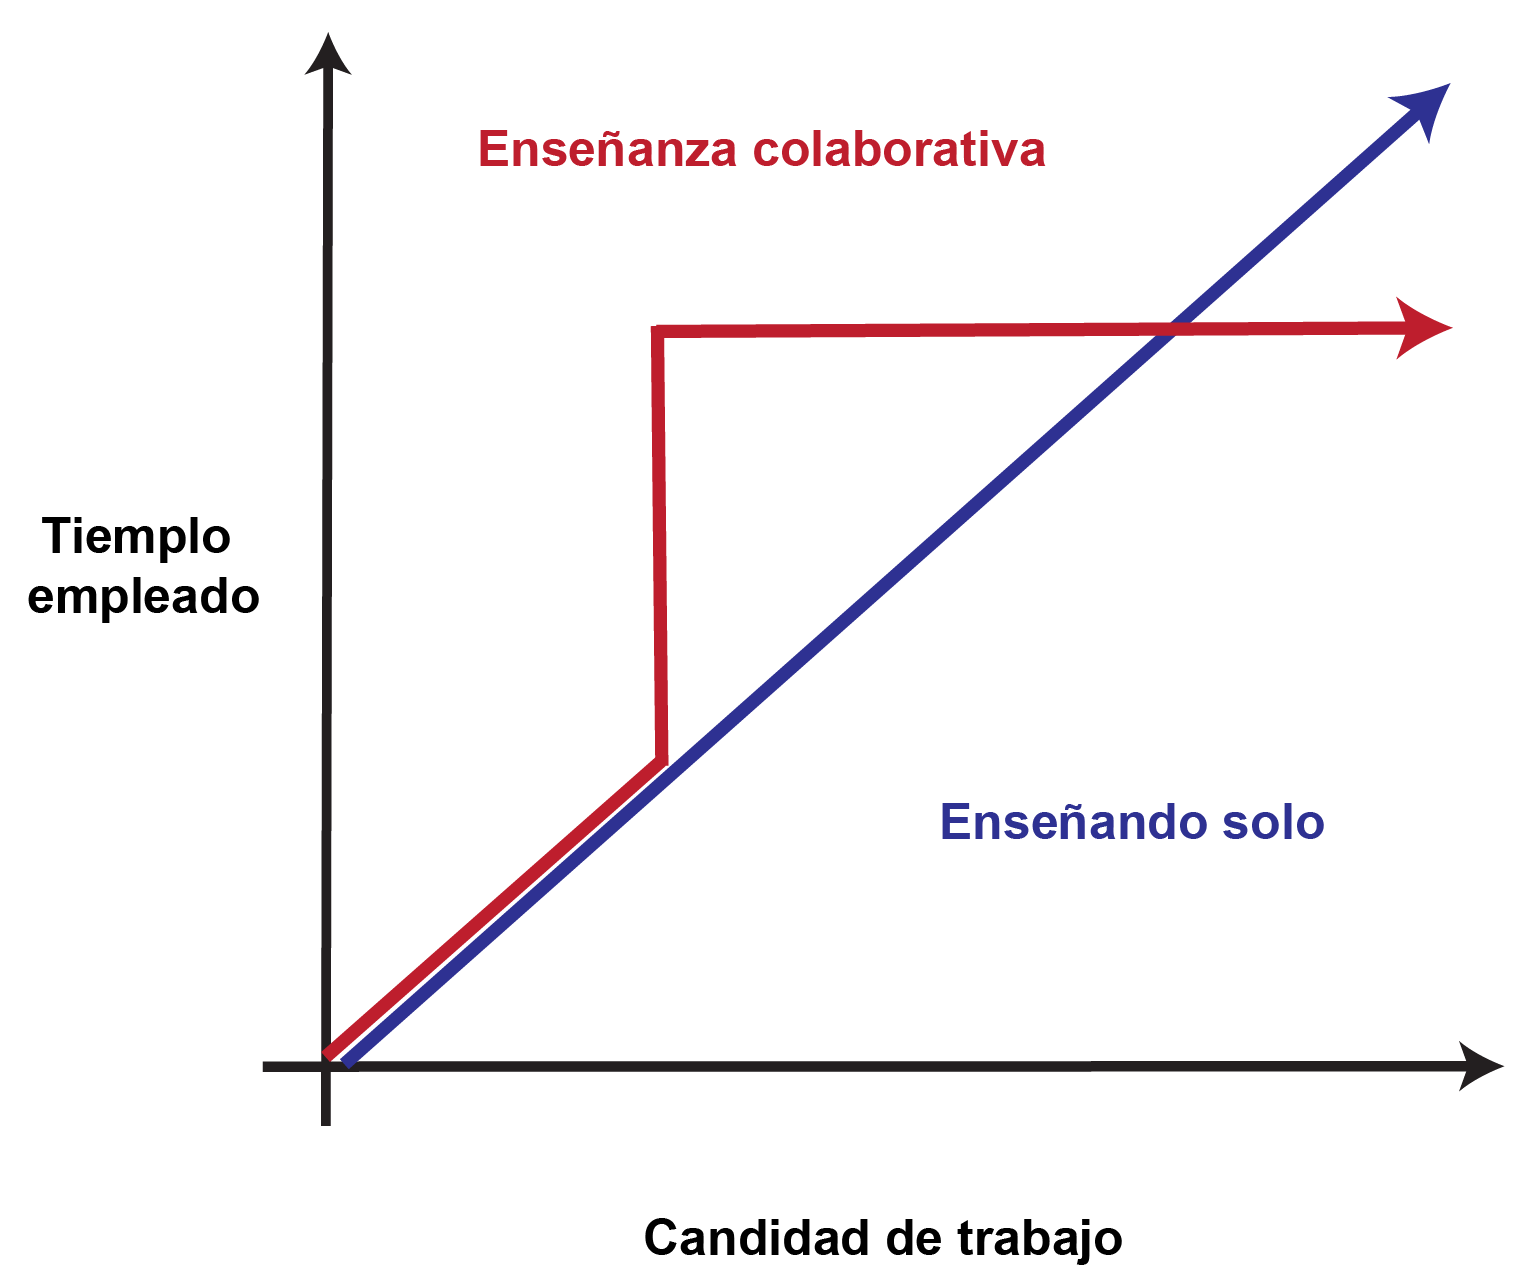
\includegraphics[width=0.75000\textwidth]{../figures/10_talk/tiempo-02.png}

\end{frame}

\begin{frame}{Consejo 1: Use \emph{R Markdown} para reproducibilidad y
familiarícese con archivos de texto sin formato}

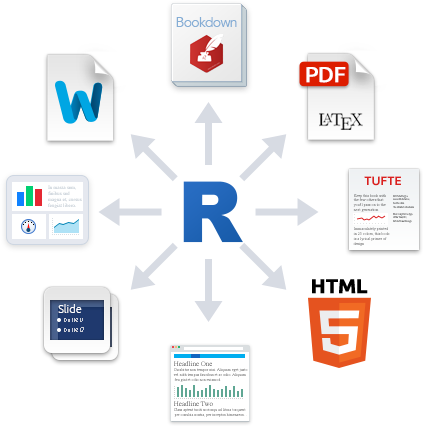
\includegraphics[width=0.50000\textwidth]{../figures/10_talk/Rmarkdown.png}
\footnote<.->{\url{https://rmarkdown.rstudio.com/authoring_quick_tour.html}}

\end{frame}

\begin{frame}{Consejo 2: Usa el control de versiones para colaborar con
otros y con vos en el futuro}

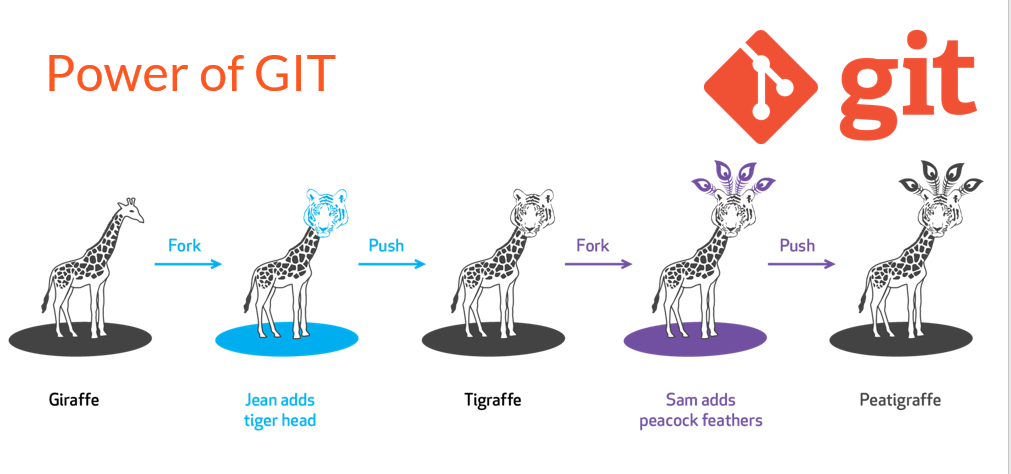
\includegraphics[width=0.75000\textwidth]{../figures/10_talk/git-graphic-01.png}
\footnote<.->{\url{http://technetnepal.net/blogs/shirishamaharjan/archive/2017/05/07/expand-horizons-change-attitudes-git-and-github-workshop.aspx}}

\end{frame}

\begin{frame}{Consejo 3: Documenta tu flujo de trabajo}

Porque probablemente sea único y complejo

\includegraphics[width=0.75000\textwidth]{https://www.blogdelfotografo.com/wp-content/uploads/2016/05/mark-516279_1920.jpg}
\footnote<.->{\url{https://www.blogdelfotografo.com/workflow-flujo-trabajo-foto/}}

\end{frame}

\begin{frame}{Ejemplo de archivo README.md}

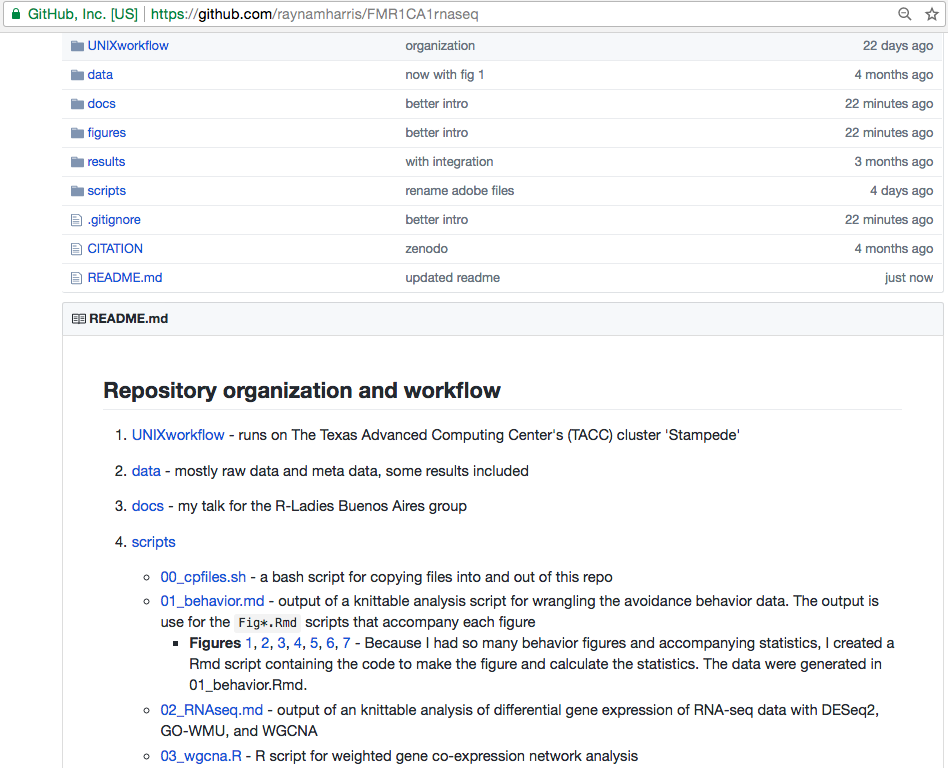
\includegraphics[width=0.75000\textwidth]{../figures/10_talk/Rworkflow.png}
\footnote<.->{\url{https://github.com/raynamharris/FMR1CA1rnaseq}}

\end{frame}

\begin{frame}{Consejo 4: Desarrolla tu propia paleta de colores}

Colorbrewer\footnote<.->{\url{http://colorbrewer2.org/}} te ayuda a
elegir colores amigables para daltónicos

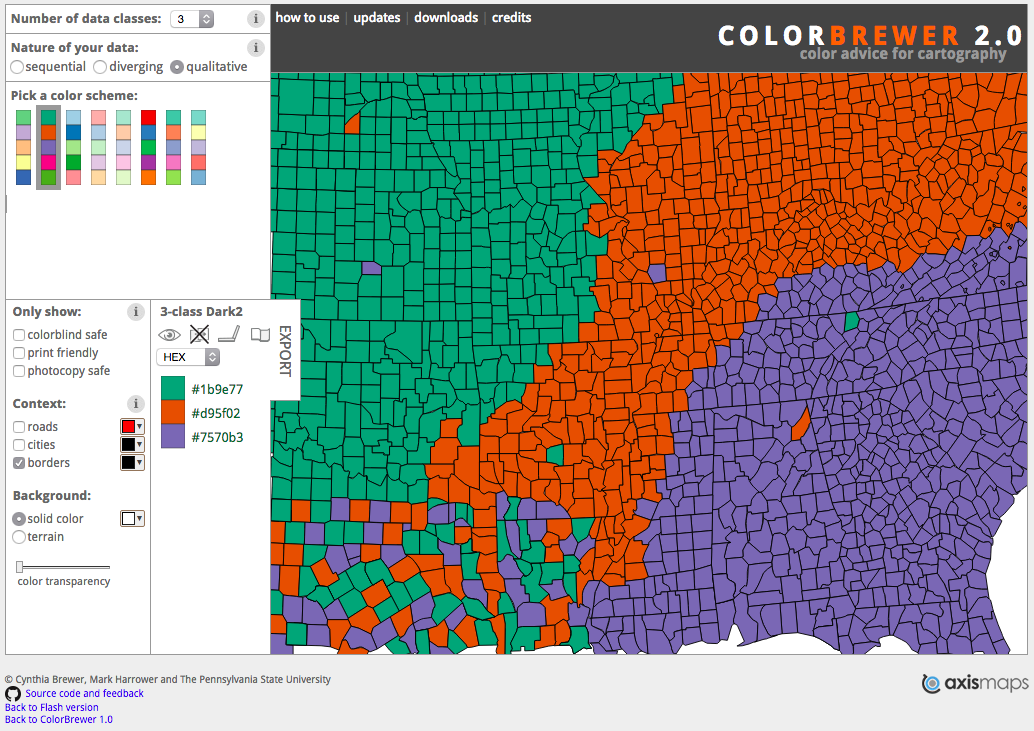
\includegraphics[width=0.75000\textwidth]{../figures/10_talk/colorbrewer.png}

\end{frame}

\begin{frame}[fragile]{Ejemplos de paletas de colores en
\texttt{ggplot}}

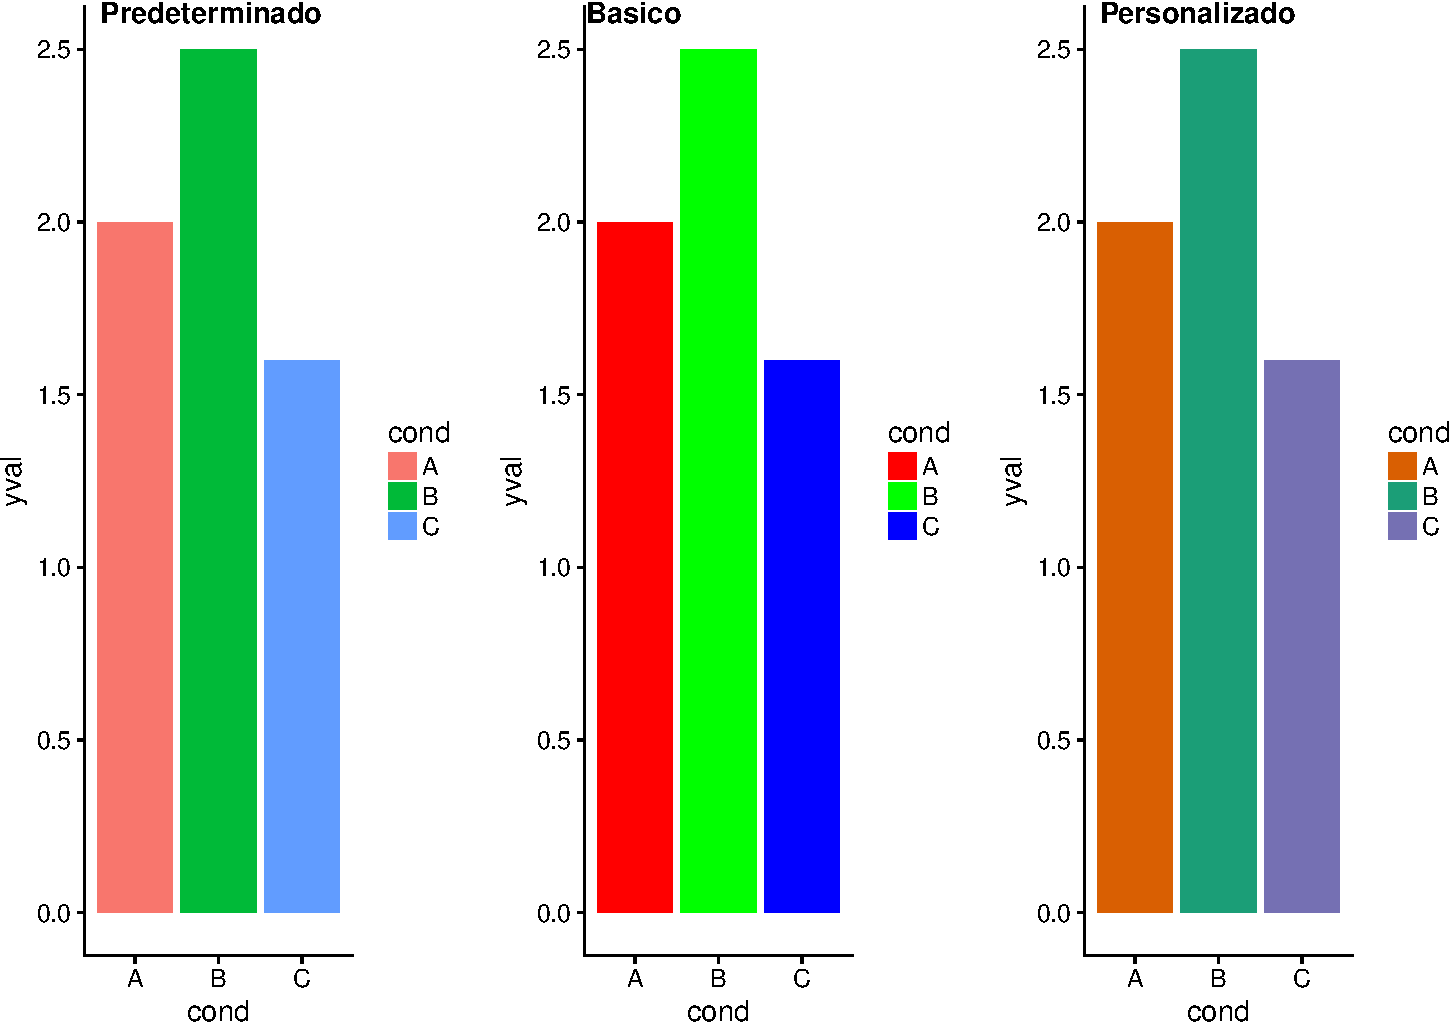
\includegraphics[width=225px]{../figures/10_talk/ejemplo-1}

\begin{itemize}[<+->]
\tightlist
\item
  Basico:
  \texttt{+\ scale\_fill\_manual(values=c("red",\ "green",\ "blue"))}
\item
  Personalizado:
  \texttt{+\ scale\_fill\_manual(values=c("\#d95f02",\ "\#1b9e77",\ "\#7570b3"))}
\end{itemize}

\end{frame}

\begin{frame}{Tu podés convertir HEX a RGB para usar la misma paletas
para las illustraciones}

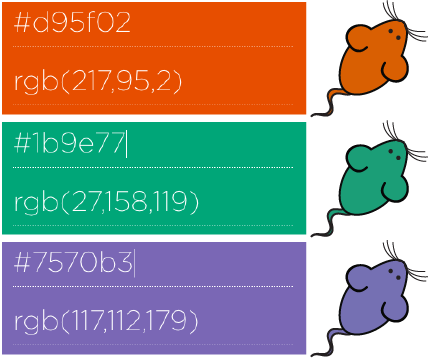
\includegraphics{../figures/10_talk/talk_colors.png} \footnote<.->{\url{https://www.webpagefx.com/web-design/hex-to-rgb/}}

\end{frame}

\begin{frame}{Consejo 5: Usa leyendas gráficas}

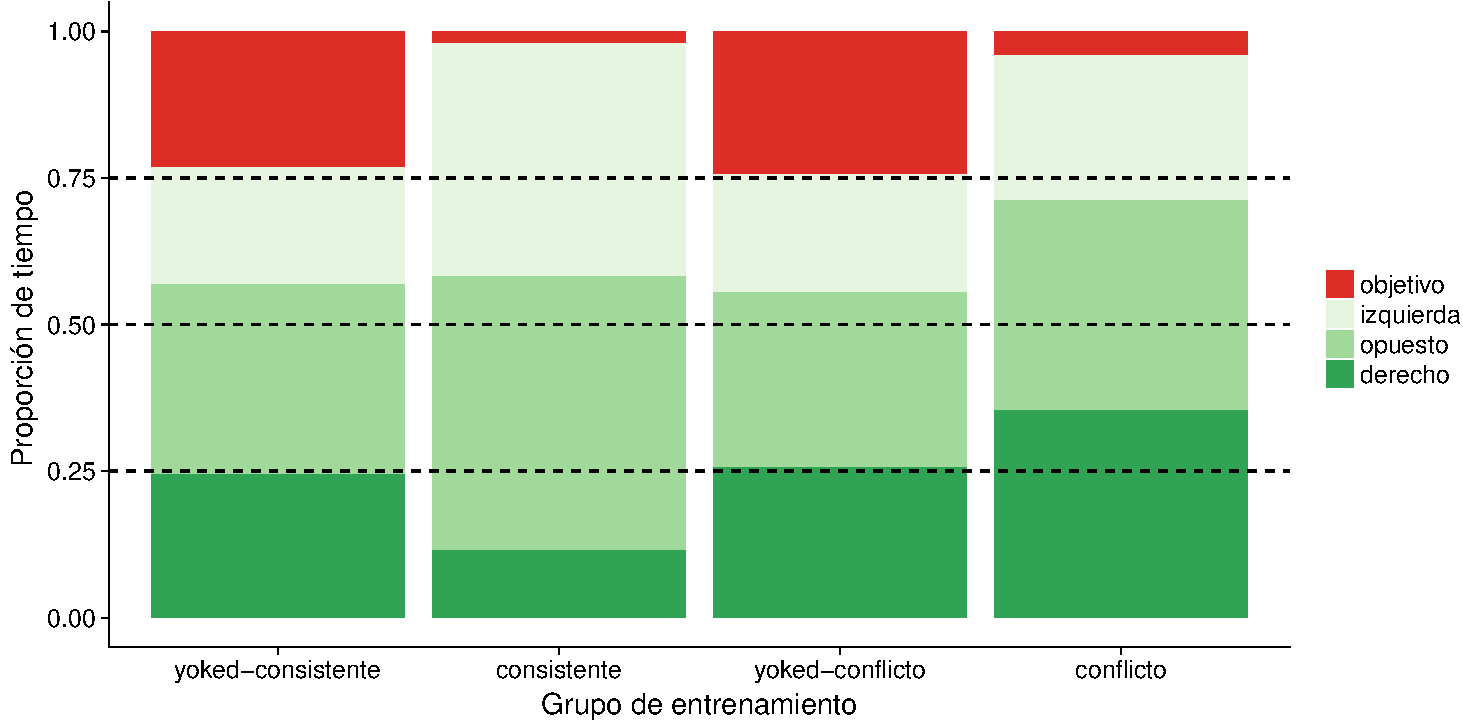
\includegraphics{../figures/10_talk/timespent-1.pdf}

\begin{itemize}[<+->]
\tightlist
\item
  Leyendas gráficas transmitir más información
\item
  Use \textbf{cowplot}\footnote<.->{\textbf{cowplot}
    \url{https://cran.r-project.org/web/packages/cowplot/index.html}}
  para agregar imágenes dentro de R
\end{itemize}

\end{frame}

\begin{frame}{Punto medio resumen}

\begin{itemize}
\tightlist
\item
  Consejo 1: Usa \emph{R Markdown} para la reproducibilidad
\item
  Consejo 2: Usa el control de versiones para la colaboración
\item
  Consejo 3: Documenta tu flujo de trabajo
\item
  Consejo 4: Desarrolla tu propia paleta de colores
\item
  Consejo 5: Usa leyendas gráficas
\end{itemize}

\end{frame}

\begin{frame}{Desarrollo colaborativo de la lección}


\includegraphics{../figures/10_talk/swc1.png}

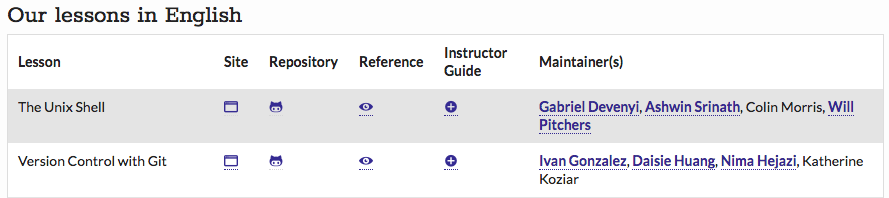
\includegraphics{../figures/10_talk/swc2.png}

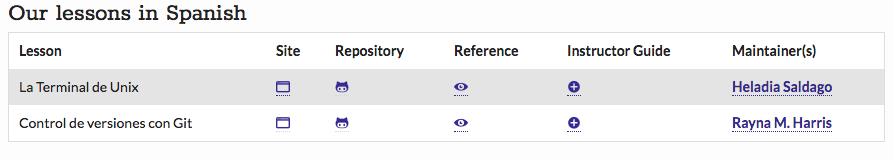
\includegraphics{../figures/10_talk/swc3.png} \footnote<.->{\url{https://software-carpentry.org/lessons/}}

\end{frame}

\begin{frame}{Deseo 1: Me ayudás a mejorar las nuevas lecciones en
español de Software Carpentry}

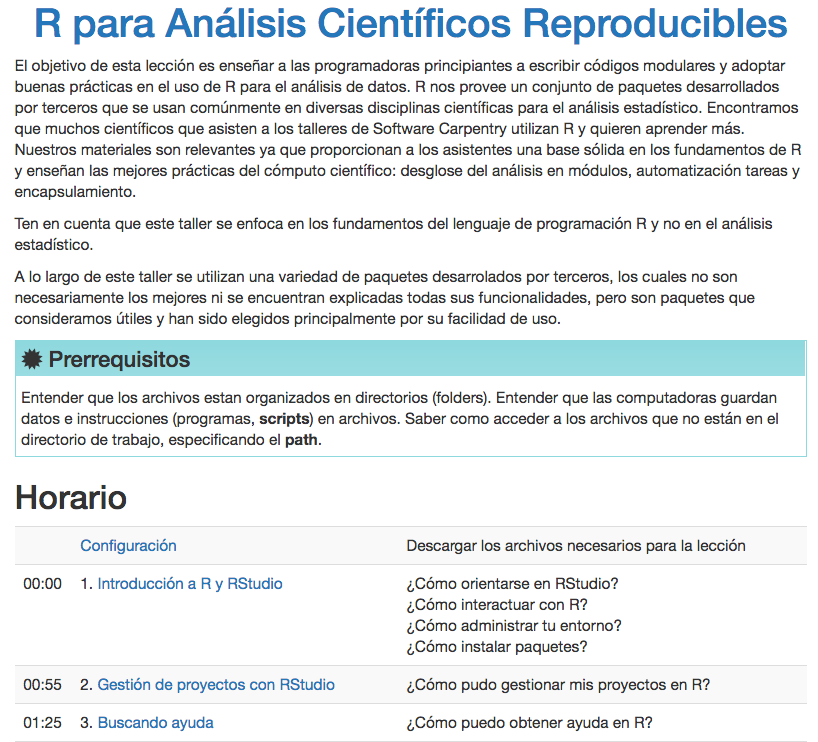
\includegraphics{../figures/10_talk/R-gapminder-es.png}

\end{frame}

\begin{frame}{Como podés ayudarme}

\begin{itemize}[<+->]
\tightlist
\item
  Leer y comentar o editar en GitHub\footnote<.->{\url{https://swcarpentry.github.io/r-novice-gapminder-es/}}
\item
  Particpar en el \textbf{Bug BBQ}\footnote<.->{\url{https://carpentries.github.io/2018-04-bug-bbq/}}
  el Abril 11 y 12
\item
  Hace videos de vos leyendo y codificando junto con la
  lección\footnote<.->{\url{https://www.youtube.com/watch?v=rQkfLaTdAvw}}
\end{itemize}

\end{frame}

\begin{frame}{Deseo 2: Convertirse en una instructora certificada}

\begin{itemize}[<+->]
\tightlist
\item
  Ahora, no hay instructoras en Argentina :(
\item
  Aplicá aquí: \url{http://carpentries.github.io/instructor-training/}
\item
  Usa el \textbf{Group Name} ``R Ladies Buenos Aires''
\end{itemize}

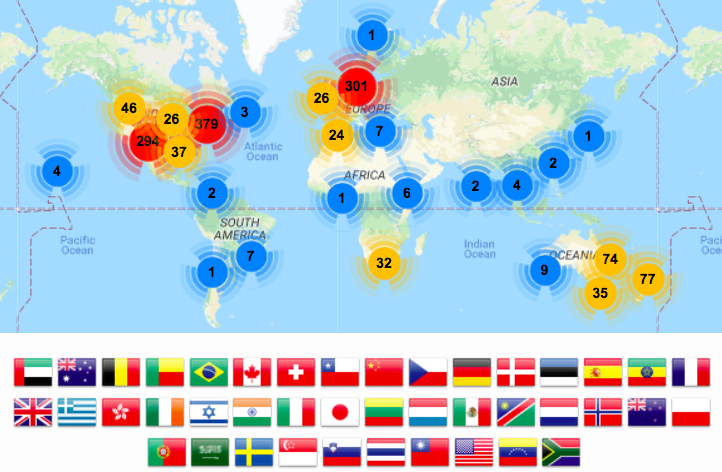
\includegraphics[width=0.75000\textwidth]{../figures/10_talk/joinus.png}
\footnote<.->{\url{https://software-carpentry.org/team/}}

\end{frame}

\begin{frame}{Deseo 3: ¡Asiste a nuestro primer taller de español!}

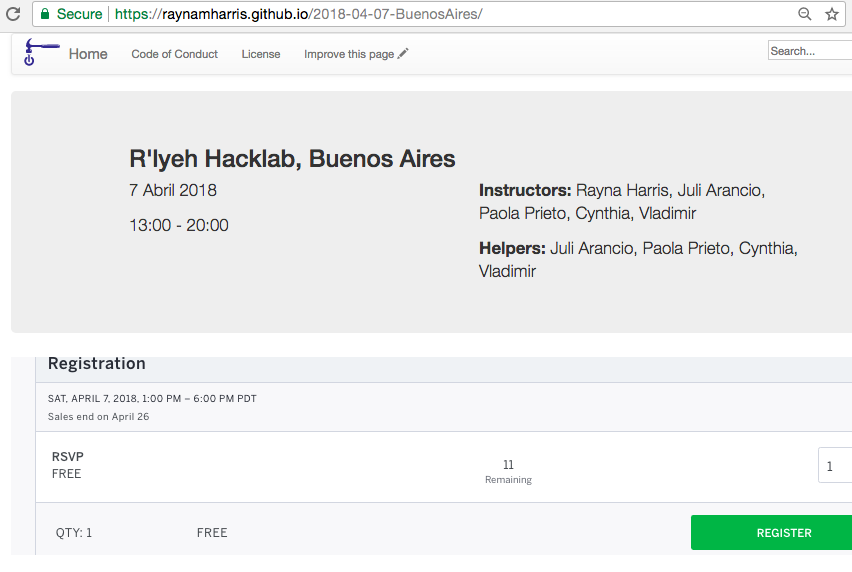
\includegraphics[width=0.75000\textwidth]{../figures/10_talk/BAtaller.png}
\footnote<.->{\url{https://raynamharris.github.io/2018-04-07-BuenosAires/}}

\end{frame}

\begin{frame}{Deseo 4: Organizar unos talleres en el futuro}

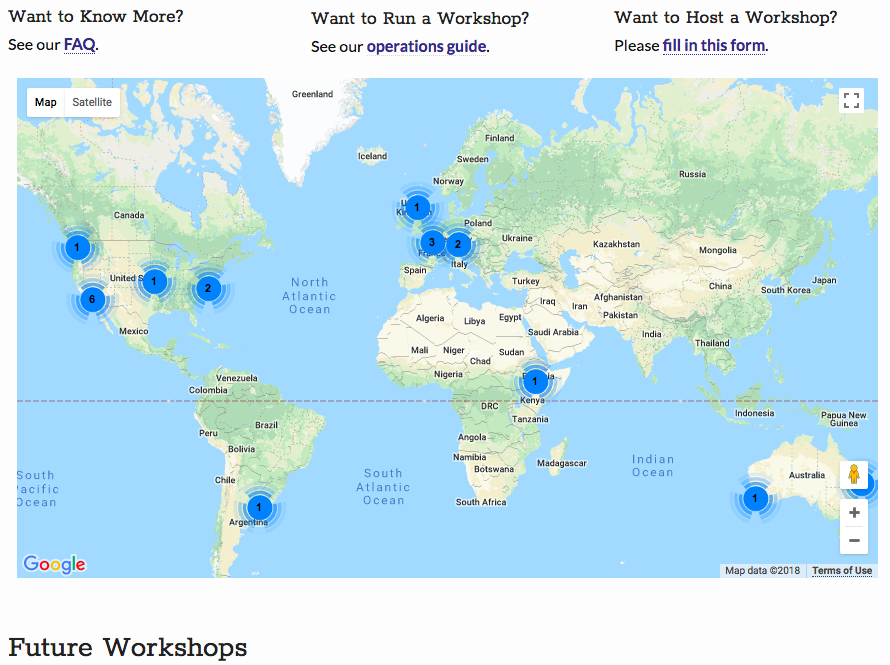
\includegraphics[width=0.75000\textwidth]{../figures/10_talk/workshops.png}
\footnote<.->{\url{https://software-carpentry.org/workshops/}}

\end{frame}

\begin{frame}{Deseo 5: Adoptar la práctica del desarrollo colaborativo
de lecciones}

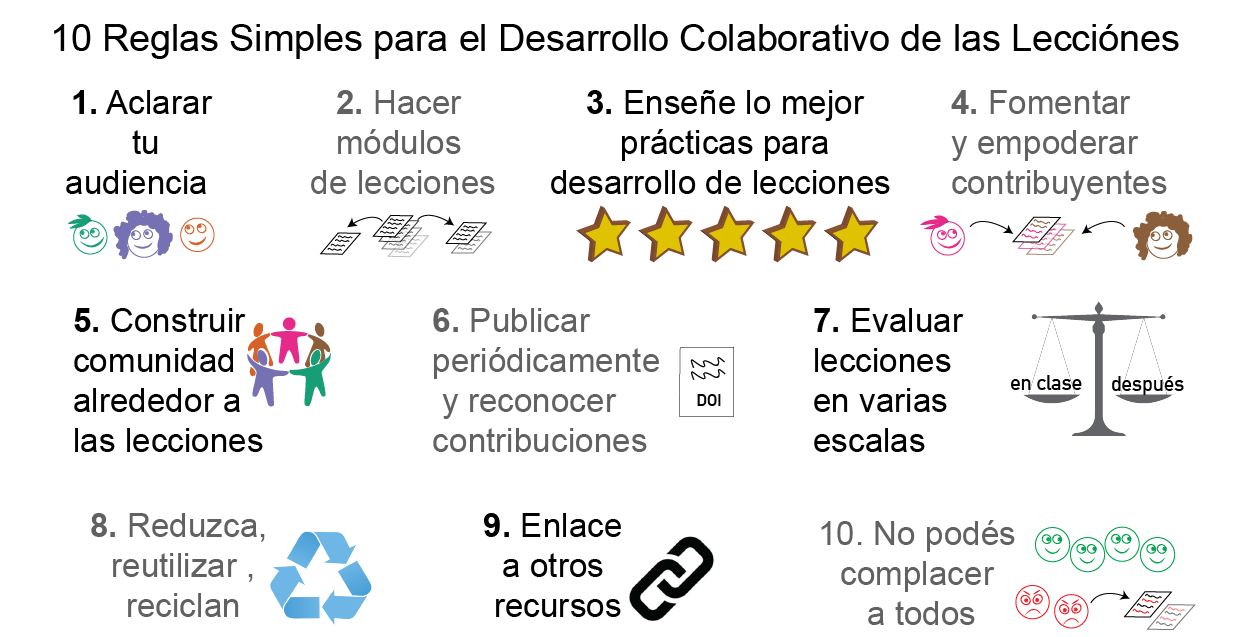
\includegraphics{../figures/10_talk/figure1_es.png} \footnote<.->{Devenyi
  et al. 2018 PLOS Comp Bio
  \url{http://journals.plos.org/ploscompbiol/article?id=10.1371/journal.pcbi.1005963}}

\end{frame}

\begin{frame}{Resumen}

\begin{itemize}
\item
  Consejo 1: Usa \emph{R Markdown} para la reproducibilidad
\item
  Consejo 2: Usa el control de versiones para la colaboración
\item
  Consejo 3: Documenta tu flujo de trabajo
\item
  Consejo 4: Desarrolla tu propia paleta de colores
\item
  Consejo 5: Usa leyendas gráficas
\item
  Deseo 1: Me ayudás a mejorar las lecciones en español
\item
  Deseo 2: Convertirse en una instructora certificada
\item
  Deseo 3: ¡Asiste a nuestro primer taller de español!
\item
  Deseo 4: Organizar unos talleres en el futuro
\item
  Deseo 5: Adoptar la práctica del desarrollo colaborativo de lecciones
\end{itemize}

\end{frame}

\begin{frame}{Pensamiento concluyente}

\begin{itemize}[<+->]
\tightlist
\item
  Yo creo que todos aprenden más cuando la ciencia y la educación está
  abiertas y reproducibles
\item
  Yo creo que la mejor manera de aprender es enseñando
\item
  Recuerda que nadie es re buena al principio, pero todas mejoramos con
  la práctica
\item
  Recuerda que vos podés hacer lo que quieras
\end{itemize}

\end{frame}

\begin{frame}{¡Gracias por tu atención! ¡Mantengámonos en contacto!}

Twitter y GitHub y Instrgram: @raynamharris

Email:
\href{mailto:rayna.harris@gmail.com}{\nolinkurl{rayna.harris@gmail.com}}

\end{frame}

\end{document}
